%% ****** Start of file apstemplate.tex ****** %
%%
%%
%%   This file is part of the APS files in the REVTeX 4 distribution.
%%   Version 4.1r of REVTeX, August 2010
%%
%%
%%   Copyright (c) 2001, 2009, 2010 The American Physical Society.
%%
%%   See the REVTeX 4 README file for restrictions and more information.
%%
%
% This is a template for producing manuscripts for use with REVTEX 4.0
% Copy this file to another name and then work on that file.
% That way, you always have this original template file to use.
%
% Group addresses by affiliation; use superscriptaddress for long
% author lists, or if there are many overlapping affiliations.
% For Phys. Rev. appearance, change preprint to twocolumn.
% Choose pra, prb, prc, prd, pre, prl, prstab, prstper, or rmp for journal
%  Add 'draft' option to mark overfull boxes with black boxes
%  Add 'showpacs' option to make PACS codes appear
%  Add 'showkeys' option to make keywords appear
%\documentclass[aps,prb,preprint,superscriptaddress,showkeys,endfloats]{revtex4-1}
%\documentclass[aps,prb,preprint,superscriptaddress,showkeys]{revtex4-1}
\documentclass[aps,prl,reprint,superscriptaddress,showkeys]{revtex4-1}
\usepackage{amsmath}
\usepackage{color}
\usepackage{graphicx}
\usepackage{dcolumn}
\usepackage{verbatim}
\usepackage{epstopdf}
\usepackage{inputenc}
\newcolumntype{d}{D{.}{.}{-1}}





\begin{document}




%\title{Fully parallel methods for calculation of partition functions for systems with known number of states with application to crystalline Li$_2$OHCl and Li$_2$OHBr}
\title{ Naturally   parallelizable and self consisent Wang and Landau  algorithm for calculation of energy density of states}

\author{Jason D. Howard}
\affiliation{Materials Science Division, Argonne National Lab, Lemont, IL, 60439, USA}

\date{\today}

%\begin{abstract}
%\input{abstract}
%\end{abstract}


\begin{acknowledgments}
\end{acknowledgments}
\begin{abstract}
In this work  an algorithm  is proposed that calculates the energy density of states, this algorithm combines random sets with Wang and Landau importance sampling  and is naturally parallelizable. The algorithm is referred to as B$_L$ENDER, which is an acronym for B$_L$end Each New Density Each Round and an  adjective for  how it was created and functions. The algorithm was developed for the purpose of working towards the goal of using first principles simulations, such as density functional theory, to calculate the partition function of disordered sub lattices in crystal materials. In this work  the algorithm is tested with the 2d Ising model as an analogous system to the disordered cubic phase of the solid state lithium ion electrolyte Li$_2$OHCl. This was done in the spirit of a ``Fermi" problem to make a prediction of the  wall time and core hours necessary for the algorithm to evaluate the partition function of a 3$\times$3$\times$3 supercell of disordered cubic Li$_2$OHCl. This work also demonstrates that, during the simulation to calculate the energy density of states, arithmetic averages of  order parameters can be made for each energy level. With these averages and the energy density of states the ensemble average of the order parameter can be determined at any temperature. 
\end{abstract}
\maketitle
For crystalline  materials  with disordered sub-lattices such as the Li-ion solid state electrolyte  Li$_2$OHCl\cite{Hood, Goodenough, Schwering, Holzwarth_group, Song_Borodin} it is desirable to calculate from first principles methods(such as density functional theory\cite{kohn:1965}) the density of energy states $G(E_j)$. Here the energy density of states is meant to correspond to the energies of the distinct lattice configurations. With the energy density of states the partition function,
\begin{equation}
\begin{split}
Z = \sum_{i}^{\Omega}e^{\frac{-e_i}{k_B T} }= \sum_{j}^{\Pi}G(E_j)e^{\frac{-E_j}{k_BT}} \;,
\end{split}
\label{partition}
\end{equation}
can be  determined and from it many important thermodynamics properties such as the free energy, entropy, specific heat, and ensemble averages calculated. In Eq. (\ref{partition}), $\Omega$ corresponds to the number of possible configurations and energies in the set $\{\Sigma_i,e_i\}_\Omega$, $\Pi$ to number of possible distinct energies $E_j$, $k_B$ is Boltzman's constant, and $T$ is the temperature. One method to solve this problem could be temperature dependent simulations involving the  Metropolis algorithm and histogram re-weighting techniques\cite{metropolis_equation_1953, landau_MC_simulations}.   Another algorithm called the  Wang and Landau algorithm\cite{WL_phys_rev_lett} has been developed which is temperature independent.  An issue with these algorithms in use with first principles methods such as density functional theory is the large number of iterations needed which would require a prohibitively long wall time at the current performance power of computers.  In this paper a method is proposed that combines the use of random sets along with the importance sampling method of the Wang and Landau algorithm that is meant to work towards the goal of highly parallel importance sampling algorithms that mesh well with high performance computing architectures. The algorithm developed in this work is referred to as the B$_{L}$ENDER (B$_{L}$end Each New Density Each Round) algorithm. The name B$_{L}$ENDER functions as an  adjective as well as an acronym. This comes from how it blends the ideas of a random set and the Wang and Landau method of sampling with probablity proportional to the inverse of the density of states, and also due to the nature of the algorithm iteratively blending histograms to produce a converged density of states.  The Wang and Landau method does have parallel versions, including  restricting random walkers to specific energy ranges or allowing the walkers to explore the entire space while periodically communicating with each other \cite{MP_Wang_Landau,P_imp_Wang_Landau, Hframe_Wang_Landau}.  The B$_{L}$ENDER algorithm is natural to parallelize as it is based on a set of random walkers that each can explore the entire energy range. 

   In practice the calculation of the energy density of states $G(E_j)$  may  is  possible through randomly sampling the configuration space $\{ \Sigma_i, e_i \}_\Omega $ of the $\Omega$.  The problem with this method is that if $\Omega$ is large, which it is for many problems,  then the computationally effort to achieve convergence is not feasible. While the methods described previously of multi canaonical sampling and the Wang and Landau algorithm tackles this issue this work aimed to produce a Wang and Landau algorithm algorithm that is highly parallel in terms of the calculation of the energies. The algorithm designed in this work is inheriently designed for the compuation of the configurational density of states of lattice models, regardless of the calculational method for the energies. In particular the algorithm produced in this work is designed for problems were the calculation of the energy is much longer than updates in the density of states. 
   
The B$_{L}$ENDER algorithm proposed in this work  is given as follows. It is noted that the following algorithm is in terms of producing a relative density of states $H(E_j)^I$, where $I$ is the iteration number. 

\begin{equation}
\begin{split}
&1.\hspace{0.125cm} H(E_j)^I ,\hspace{0.15cm}  \{\Sigma_{s},e_s\}_{\mathcal{S}}^I\\
&2. \hspace{0.125cm}\{\Sigma_{s},e_s\}_{\mathcal{S}}^I \rightarrow  \{\Sigma_{s}^{'},e_s^{'}\}_{\mathcal{S}}^I\\
&3. \hspace{0.125cm} \Sigma_{s}^{'I}, e_s^{'I} \rightarrow \Sigma_{s}^{I+1},e_s^{I+1}   \hspace{0.125cm} P = \hspace{0.075cm} min [1, H(e_s)^{I}/H(e_s^{'})^{I}]\\
& \hspace{0.125cm}else  \hspace{0.15cm} \Sigma_{s}^I, e_s^I \rightarrow \Sigma_{s}^{I+1}, e_s^{I+1}\\
&4. \hspace{0.125cm} H(E_j)^{I+1} =  \\
& H(E_j)^{I} + \frac{C_o \mathcal{H}(E_j,\{e_s\}_{\mathcal{S}}^{I+1}) }{ [\sum_j H(E_j)^{I}]^{\frac{1}{N} } }H(E_j)^{I} = \\
& H(E_j)^{I}( 1 +  \frac{C_o \mathcal{H}(E_j,\{e_s\}_{\mathcal{S}}^{I+1}) }{ [\sum_j H(E_j)^{I}]^{\frac{1}{N} } } )\\
\end{split}
\label{blender}
\end{equation}
Where  $H(E_j)^0 \equiv [1 +  \frac{C_o}{S}\mathcal{H}(E_j,\{e_s\}_{\mathcal{S}}^0)]$ with $\mathcal{H}(E_j,\{e_s\}_{\mathcal{S}})$ being a histogram function that counts the number of energies $E_j$ in the set $\{e_s\}_{\mathcal{S}}$. In this work $\{\Sigma_{s},e_s\}_{\mathcal{S}}^0$  is a randomly(uniformly) drawn set from the configuration space $\{ \Sigma_i, e_i \}_\Omega $. In the second step  a random change is applied to each element of the sampled set $\{\Sigma_{s},e_s\}_{\mathcal{S}}^I$ to produced a ``perturbed" set $ \{\Sigma_{s}^{'},e_s^{'}\}_{\mathcal{S}}^I$ , for the Ising model this could be randomly flipping a spin.  In the third step a random number is drawn between zero and one for every sampled configuration, if this number is less then the ratio of the current density of states $H(e_s)^{I}/H(e_s^{'})^{I}$ then the perturbed configuration and energy  $\Sigma_{s}^{'I},e_s^{'I}$  goes to $\Sigma_{s}^{I+1},e_s^{I+1}$,  else the unperturbed configuration and energy $\Sigma_{s}^{I},e_s^I$  goes to $\Sigma_{s}^{I+1},e_s^{I+1}$. This step (third) is dervied from the Wang and Landau method of sampling with probablity proportional to the inverse of the density of states.  In the fourth step a histogram of the updated $\{ e_s \}^{I+1}_{\mathcal{S}}$ energies is made and added (blended) in to the current density of states $H(E_j)^I$   by multiplying  by a constant $C_{o}$(which affects the convergence properties) and the relative probability of each energy $E_j$ in the  intermediary density of states $H(E_j)^{I}$. The fourth step is also shown in terms of multiplication which is discussed later. In this work it was found  $C_{o}=\Omega^{\frac{1}{N}}$ was computationally efficient. After the algorithm is deemed to be complete it is necessary to re-normalize the iterated relative density of states $H(E_j)^f$ at the final iteration $I=f$ as follows, 
\begin{equation}
\begin{split}
&1. \hspace{0.125cm} A = \sum_jH(E_j)^f\\
&2. \hspace{0.125cm} G(E_j)\approx H(E_j)^f \frac{\Omega}{A} \;,
\end{split}
\end{equation}
to produce the properly normalized estimated value of $G(E_j)$. 

An important discussion point of this algorithm (Eq \ref{blender}) is the update of the relative density(step four) of states being presented as addition and multiplication. In the addition form the self consistent nature of the update is clear, in the sense that the  density of states is updated by adding a  piece proportional to the counts in the histogram of the random set times the relative proportion of  that energy level in the current estimate of the density of states.  In the typical Wang and Landau sampling the update of the density of states is preformed by multiplication combined with a periodic reduction of the multiplication factor. In the multiplication form of step four of this algorithm (Eq \ref{blender}) it is seen that the dependence on one over the sum of the density of states serves to naturally reduce the multiplication factor as the simulation progresses. The multiplication form is also useful when $\Omega$ is large and the sum of the density of states is larger than a typical floating point number. In this case the log of the density of states can be stored and the update performed through addition of logs. Taking $H_M \equiv  max[H(E_j)]$ the log of $\sum_j H(E_j)^{I}$ can be written as, 
\begin{equation}
\begin{split}
&H_{LS} \equiv \log[\sum_j H(E_j)^{I}] = \log[H_M \frac{\sum_j H(E_j)^{I}}{H_M}]=\\
&\log[H_M] + \log[\sum_j e^{\ln[H(E_j)] - \ln[H_M]} ] \;.
\end{split}
\label{Hls}
\end{equation} 
With $H_{LS}$ from Eq \ref{Hls} the $\log$ update form of step four of the algorithm (Eq \ref{blender}) can be written as the following, 
\begin{equation}
\begin{split}
& \log[ H(E_j)^{I}( 1 +  \frac{C_o \mathcal{H}(E_j,\{e_s\}_{\mathcal{S}}^{I+1}) }{ [\sum_j H(E_j)^{I}]^{\frac{1}{N} } } ) ]=\\
& \log[ H(E_j)^{I} ] + \log[1 +   \mathcal{H}(E_j,\{e_s\}_{\mathcal{S}}^{I+1})e^{\ln[C_o]-\frac{1}{N}H_{LS}}] \;.
\end{split}
\end{equation}
In this form  the alogrithm can be implemented even when $\Omega$ is large. To implement the ratio of the density of states in step two of the algorithm, 
\begin{equation}
e^{\ln[H(e_s)^{I}] - \ln[H(e_s^{'})^{I}]} \;,
\end{equation}
can be used.

In this work the algorithm discussed is tested using the 2d square zero field  Ising model with lattice dimension of even number\cite{exact_statistical,Onsager,Ising}.  The configurations $\Sigma_i$ and energies $e_i$ of the 2d Ising model are inherently defined by the lattice site spin variables and coupling constant $J$.   The first test is a test the effectiveness of the algorithm in calculating the density of states of the 2-d ising model. . To test the accuracy of the simulations the results will be compared to the exact result solved by Beale \cite{Beale_2d_ising}. The accuracy of the simulation will be determined by the average of errors given as, 
\begin{equation}
\begin{split}
 &\mathcal{E}(I,o) \hspace{0.1cm}= \hspace{0.1cm}< |\epsilon(E_j,I,o)| >_j\\
& = \hspace{0.1cm}  \frac{1}{\Pi} \sum_{j=1}^{\Pi}\frac{|\ln(G_{ex}(E_j))- \ln(G_{cal}(E_j,I,o))|}{|\ln(G_{ex}(E_j))|}\; 
 \end{split}. 
 \label{avg_error}
\end{equation}

Where $G_{ex}(E_j)$ is the exact density of states, $G_{cal}(E_j,I,o)$ is the calculated density of states  at iteration number $I$ from initial conditions and trajectory $o$, and $|\epsilon(E_j,I,o)|$ is the absolute value of the fractional error for a specific energy level.  This first test of the algorithm is with the 32X32 Ising model. While the ideal value of $N$ is not known a-priori it was found in this work that a values of $N=0.1$ was computationally efficient for the 32X32 Ising model. In Fig \ref{thirtytwo_Stest} the value of the average error calculated with Eq \ref{avg_error} is shown up to 1e7 iterations for $S=1$ , $10$, $100$, $1000$, and $1e4$. The data in Fig \ref{thirtytwo_Stest} is averaged over 36 individual simulations for each value of $S$. The results show linear scaling from $S=1$ to $S=10$ and then another order of magnitude improvement from $S=10$ to $S=1000$, no improvement is discernable going to $S=1e4$.  The flucuations in the avg error are also noted in going to larger $S$. The results at $S=1000$ show that the average error is comparable to a linear speed up of the error reported for a single random walker in the orignial Wang and Landau algorithm. Defining a effective Monte Carlo step defined here as,

\begin{equation}
MC = \frac{S\times I}{\#E} \;,
\end{equation} 
where $\#E$ is the number of energies. For $S=1000$, with the number of energies for the 2-d Ising model given by $n\times n$, at $I=1e7$ gives $MC \approx 1e6$. With the value of the average error being $<0.001$ for $S=1000$ at $MC\approx 1e6$ the B$_L$ENDER algorithm is performing very well in terms of parallel speed up as compared to the reports for the orignial Wang and Landau algorithm for a single Walker.   
\begin{figure}
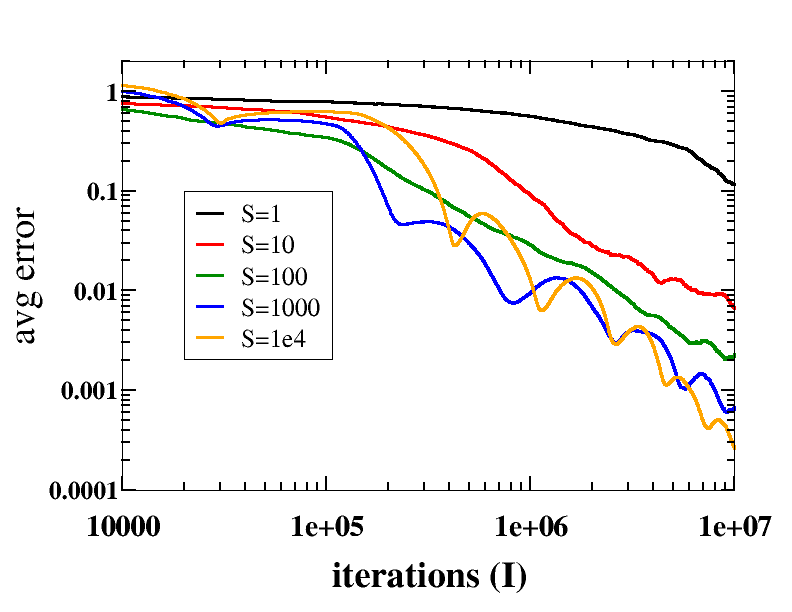
\includegraphics[width=7.5cm]{./figures/thirtytwo_root0_1_varyS.png}
\caption{\label{thirtytwo_Stest}}
\end{figure}


In a previous study\cite{partition} uniform sampling was used with first principles simulations to approximate the partition function for a $2\times 2\times 2$ supercell  of disordered cubic Li$_2$OHCl. In going to just a $3\times 3\times 3$ supercell the value of $\Omega$ would jump from $\sim 1e7$ to  $\sim 1e27$. So computing the partition function for the $3\times 3\times 3$ system of disordered cubic Li$_2$OHCl is completely intractable from uniform sampling. In this work a $10X10$ 2d Ising model with $\Omega = 1.3e30$ is used as an analogous system to predict the computational effort needed for the B$_L$ENDER algorithm to compute the partition function of a  $3\times 3\times 3$ supercell of disordered cubic Li$_2$OHCl.

 Now from Fig. \ref{its_to} (a) we could take $\mathcal{S}=100$  as an approximate optimal value to attempt a calculation of the density of states of disordered cubic Li$_2$OHCl. In willing to accept $\mathcal{E}=10\%$ there is an approximate 10$\times$ reduction in the number of iterations. So for an accuracy of $\mathcal{E}=10\%$ that gives an approximate number of iterations  $\sim 1e4$. Using the VASP code\cite{Vasp1,Vasp2,Vasp3,Vasp4} with the projector augmented wave formalism\cite{Blochl, pawVasp} and the GGA-PBE exchange and correlation functional\cite{PBE,PBEerratum}, the calculation of a structural relaxation to obtain the energy for a given lattice configuration is on the order of 2 hours for a 36 core broadwell node. So to compute the parition function of the disordered cubic lattice of a $3\times 3 \times 3$ supercell model of Li2OHCl with 100,  36-processor broadwell nodes, at the level of static lattice internal energies (no phonon free energies) calculated with GGA-PBE  would require approximately  70 million core hores and a wall time of 800 days.   So at the current moment it is still  too large of a computational effort to make utilizing this algorithm on a $3\times  3 \times 3$ model of the Li$_2$OHCl system feasible but if Moore's law continues within a decade it may be a viable option. It must be stated that this estimation on the computational effort required for the Li$_2$OHCl system is presented in the spirit of a ``Fermi" problem and is only meant for a coarse estimate and that a more detailed analogous model would be required to improve the prediction. A more detailed anlagous model might include using a 3d Ising model with fixed concentration of up and down spins and including longer range interactions. The benefit of the square 2d Ising model in this work is the availability of exact solutions to test the profficiency of the algorithm. Aside from the difficulties in large supercell first principles simulations the algorithm could be used with first principles on smaller systems, with model Hamiltonians, or systems defined by classical potentials.  


 

In summary the presented algorithm in this work has shown its effectiveness in accurately determining the density of states for the 2d square zero field Ising model.  The simulations suggest that within a decade using the B$_L$ENDER algorithm  it will be feasible on a state of the art super computer to calculate the partition function of a 3$\times$3$\times$3 135 atom model of disordered cubic Li$_2$OHCl at the static lattice internal energy level using  density functional to a high level of accuracy. At the present time the algorithm should be suitable for first principles methods with smaller system sizes, with model lattice Hamiltonians, or with models defined through classical potentials. The algorithm shows promise for first principles methods in particular because the calculation of the energies can be done as individual job submissions to compute nodes managed by a script running on a head node. This work also demonstrated that if during the simulation to determine the energy density of states, arithmetic  averages of order parameters are made for each energy level, then calculation of order parameters at any temperature is feasible.
 
\begin{acknowledgments}
This work was supported by the Center for Electrical Energy Storage: Tailored Interfaces, an Energy Frontier Research Center funded 
by the US Department of Energy, Office of Science, Office of Basic Energy Sciences at Argonne National Laboratory under Contract DE-AC02-06CH11357.
I would like to thank the Laboratory Computing Resource Center (LCRC) faculty of Argonne National Lab for their support and maintenance of the computing resources that made this project possible. 
\end{acknowledgments}
%\newcommand{\bibdir}{./}
\bibliography{Bib}
\bibliographystyle{unsrt}
\end{document}
